\section{Result of the Implementation}
\subsection{Quality Measures and Interpretation}
\begin{figure}
    \centering
    \begin{tabular}{c c}
        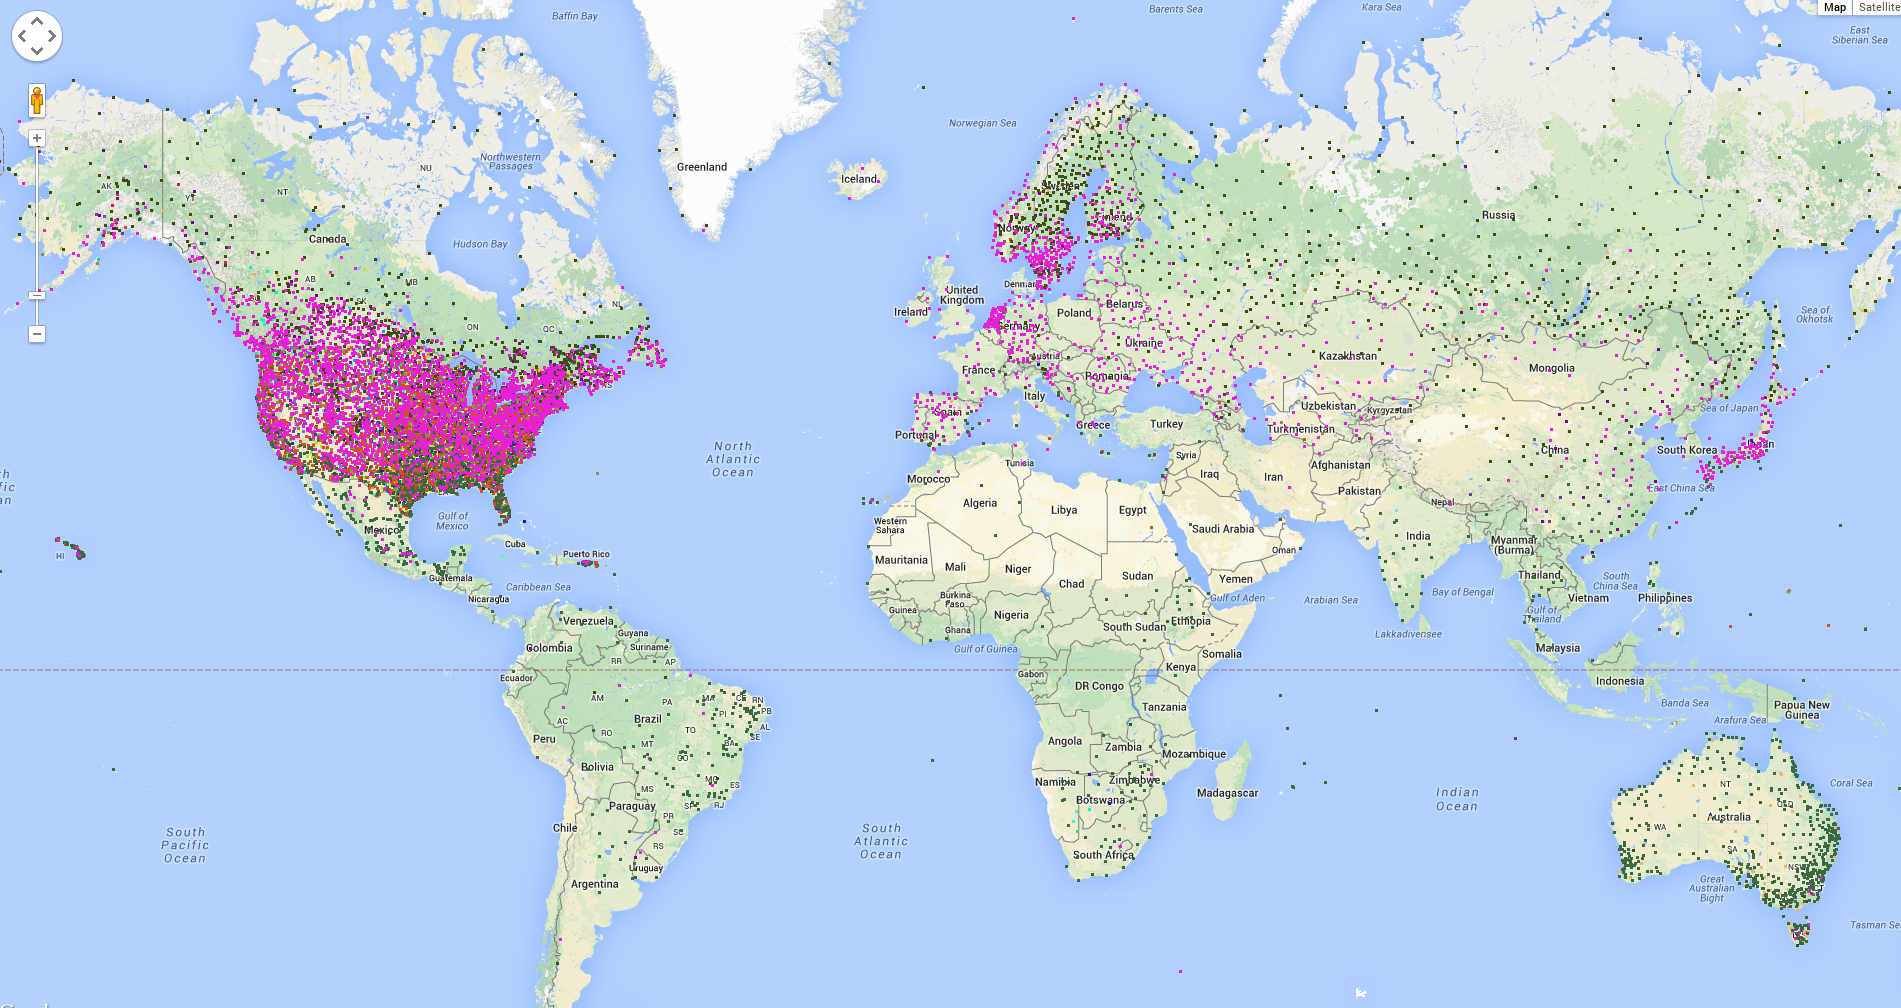
\includegraphics[width =.4\linewidth]{figure/1983.png} &         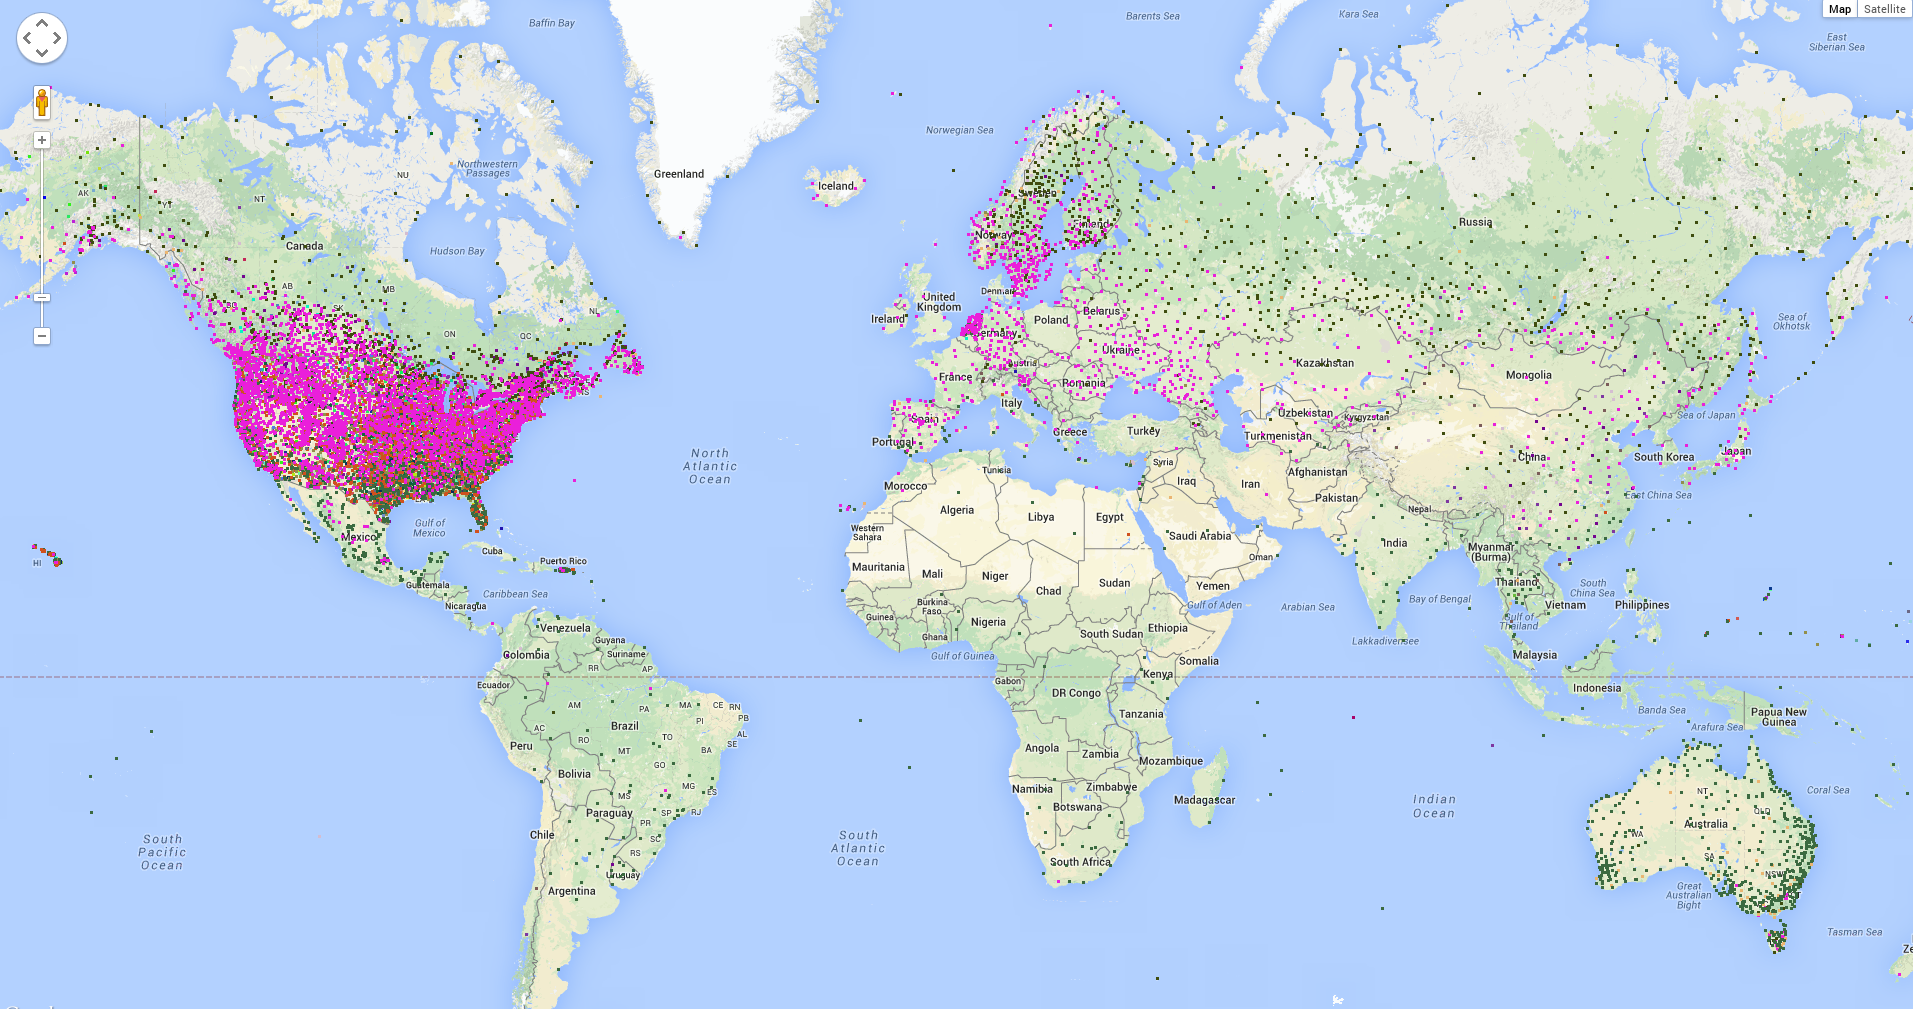
\includegraphics[width =.4\linewidth]{figure/1993.png} \\
        1983 & 1993 \\
        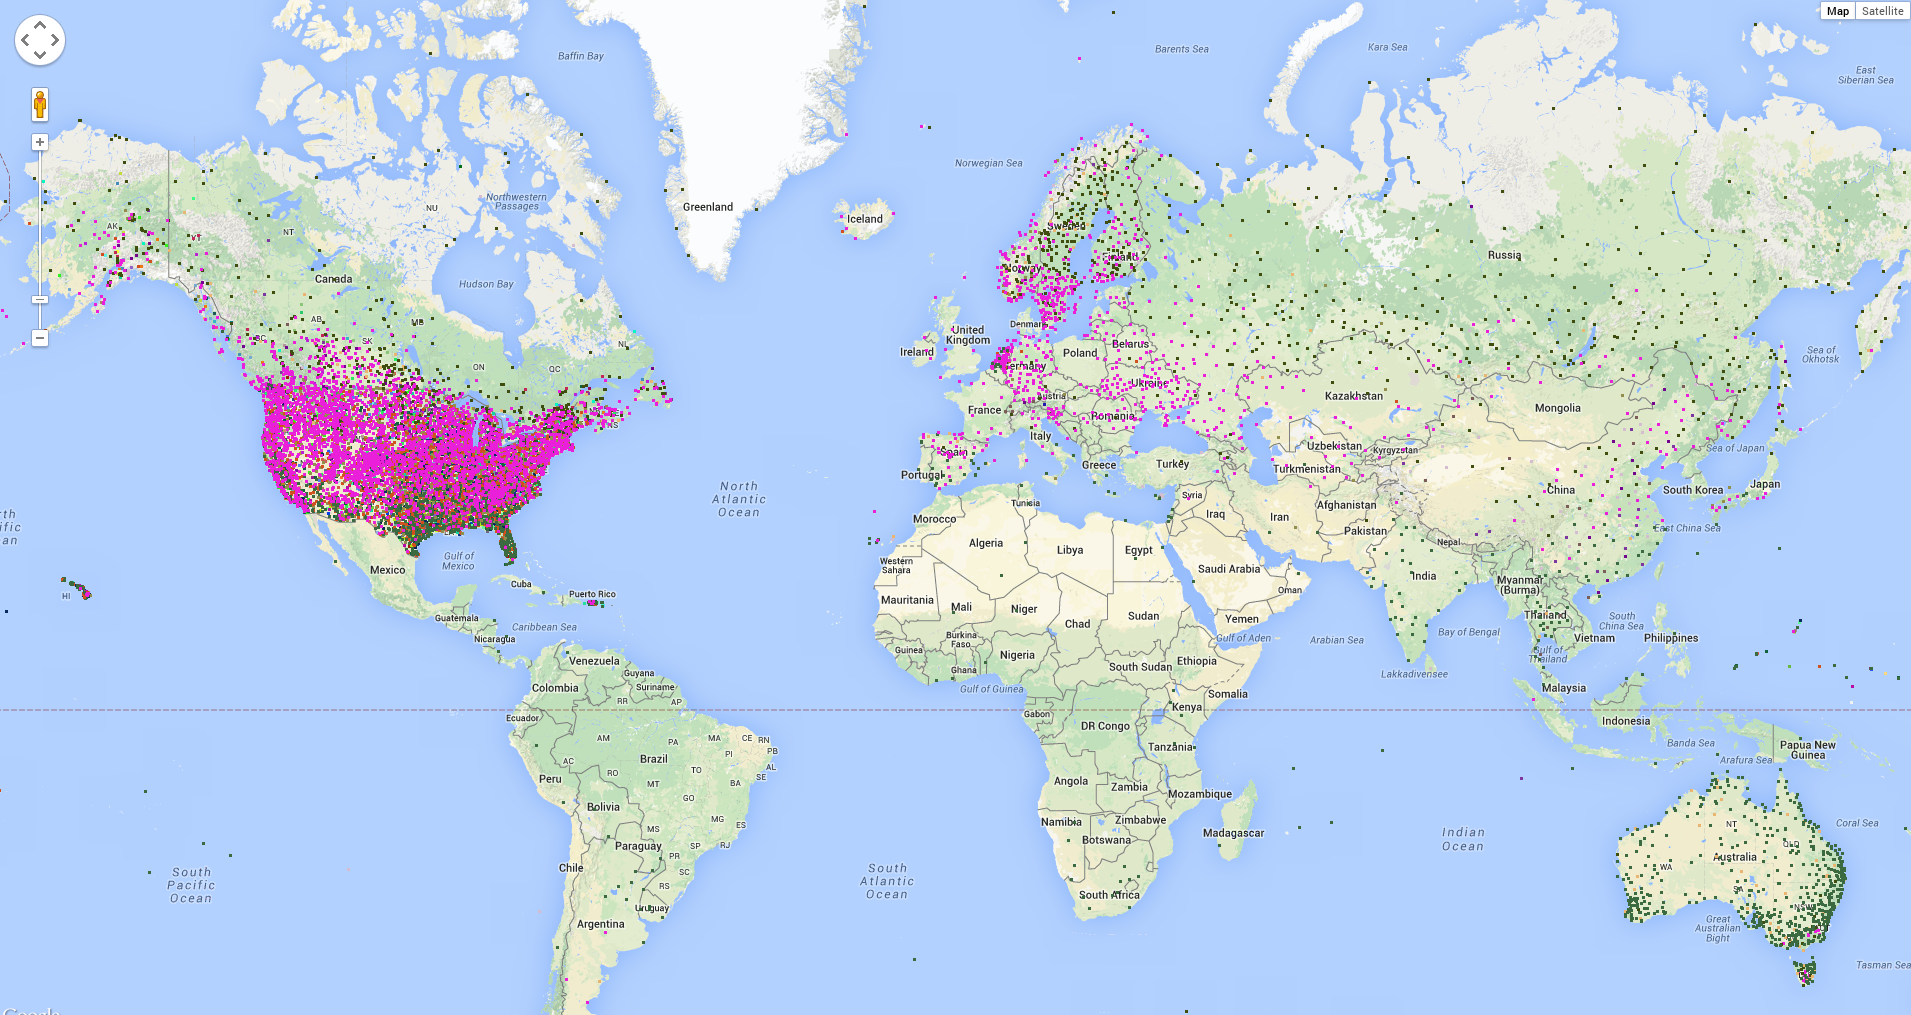
\includegraphics[width =.4\linewidth]{figure/2003.png} &         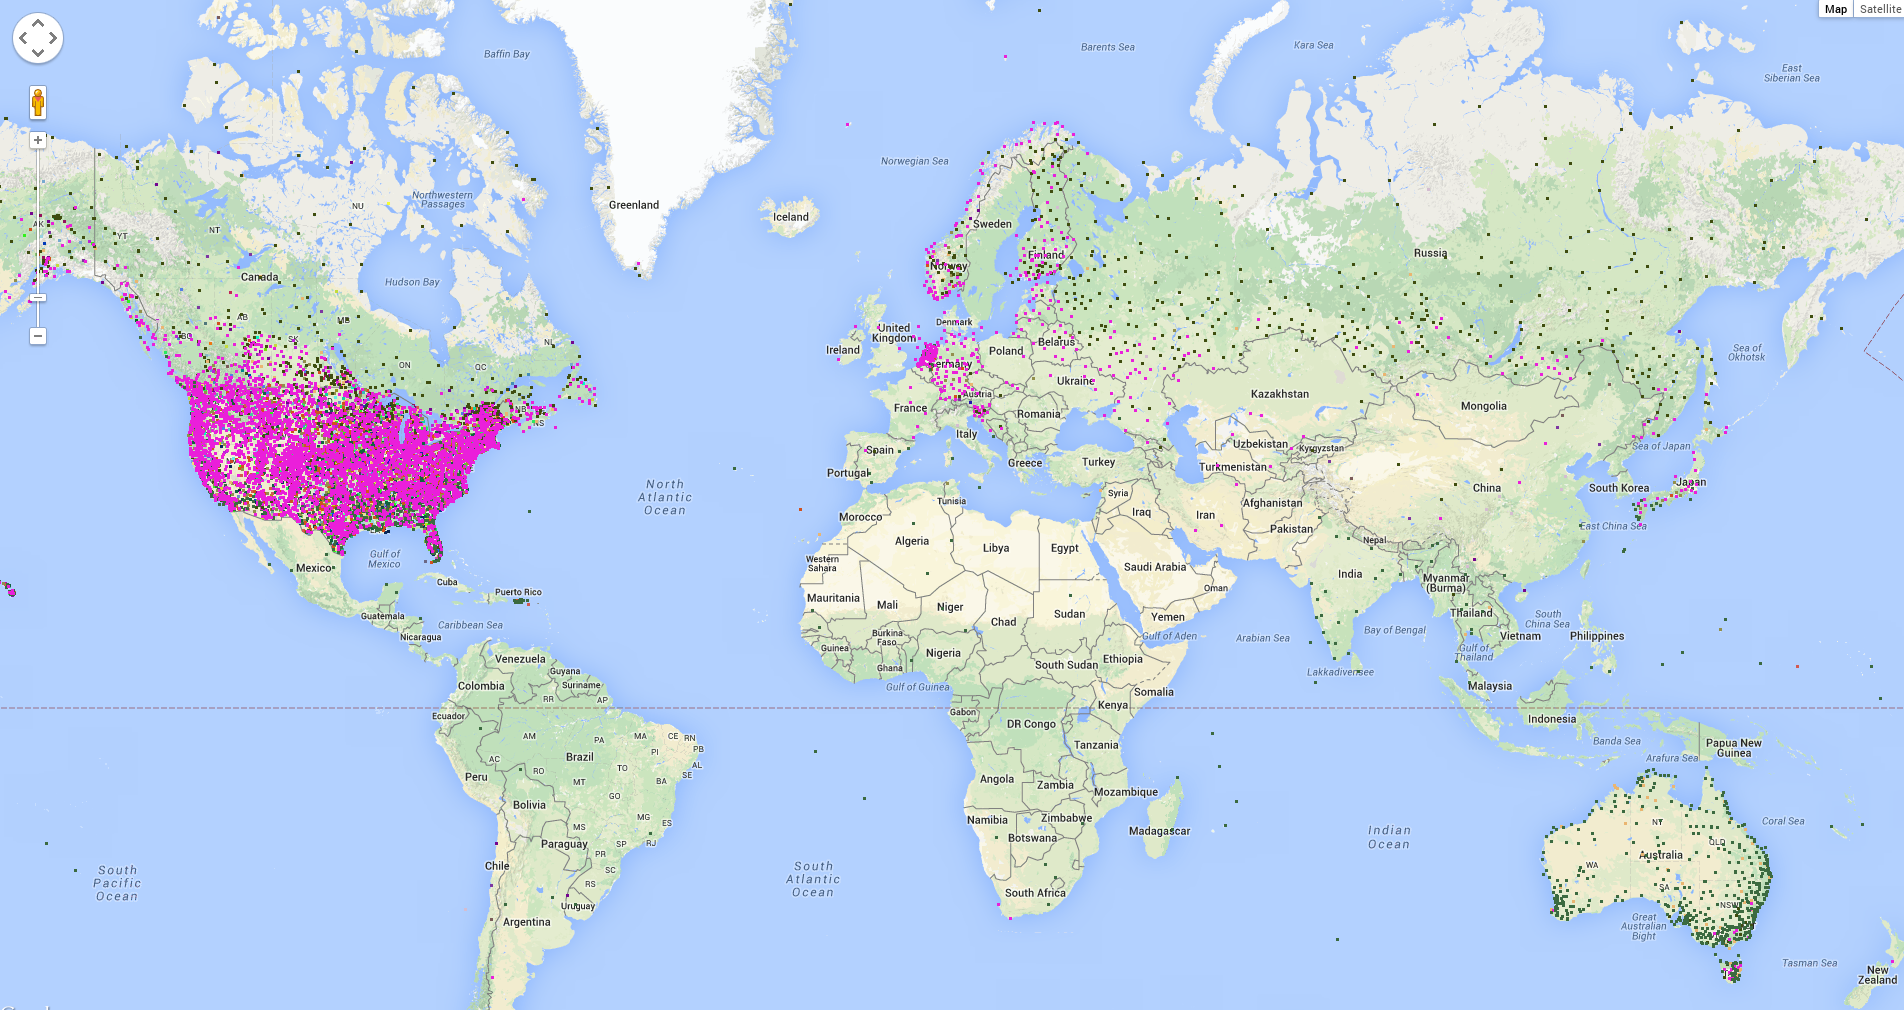
\includegraphics[width =.4\linewidth]{figure/2013.png} \\
        2003 & 2013
    \end{tabular}
    \caption{Clustering results of different years.}
    \label{fig:ClusteringFlow}
\end{figure}

From the clustering flow spanning over 4 decades in Fig \ref{fig:ClusteringFlow}, we are still not satisfied with the current results. In the following, we will discuss a few aspects of the visualization, as well as analysis with possible solutions in the next stage.

From the results, we can see there are only 3 big clusters (Majority of North America, Asia and Russia, Region around Florida) even if we set the number to be 300 for Kmeans. It does not align well with our prior geology knowledge and expected results. There are several possible reasons for this results:

1. We are eliminating data points whose features have relatively large number of missing values. Our threshold might be improper right now. For example, we can observe few points in China while there do exists much more data points in the raw data. It exerts the potential risk of removing possible climate clusters where monitoring data are not complete in all of the five measurements.

2. As we employ uniform sampling to generate coreset, we are still making efforts to analyse 2 specific distributions: (1) distribution of  numbers of data points represented by each coreset point. (2) distribution of numbers of data points represented by each cluster in coreset. If this distribution is close to uniform distribution, it means points in coreset represent unbalanced neighborhood. Then we can conclude our sampling strategy might be improper. We will adjust our sampling strategy and parameters to improve the result quality before the next milestone.

However, there are also some encouraging points in the current results. From the flow from 1983 to 2013, we can observe the three biggest clusters covering roughly the same areas with minor difference. It is a good indication that similar year-wise climate patterns are clustered into the same cluster. 

We will make efforts in verifying the correctness of sampling strategy, validity of features and different parameter. We expect better results before the last milestone. 

\subsection{Scalability}
For our feature generation tasks, we employ the following EMR master-slave pair for computation. A m3.2xlarge machine with 8 cores and 30GB memory is deployed as the master server, 2 m1.xlarge machines with 4 cores and	15GB memory are employed as slave clients. The running time and peak memory consumption for different feature generation task is summarized in the following table.

\begin{table}[H]
    \begin{tabular}{| c | c | c | c |}
    \hline
    Task & running time & peak memory & normalized instance hour \\
    \hline
    \hline
    Extract feature with missing value & 3h45min & 25GB & 124h\\
    \hline
    Calculate mean and variance of features & 40min & 25GB & 31h\\
    \hline
    Fill missing values and normalize features & 3h47min & 25GB & 124h\\
    %\hline
%    Recalculating mean and variance for normalization &  &  &\\
%    \hline
%    Feature normalization &  &  & \\
    \hline
    \end{tabular}
    \caption{Scalability performance of tasks related to feature generation.}
    \label{tbl:PerfTable}
\end{table}

As we meet difficulties in installing scikit learn library with bootstrap script when launching clusters. We set up Hadoop 2.5.2 environment on a local machine with a quad-core i5-4570 3.2Ghz processor and 16 GB memory. To meet the memory requirement for running intensive tasks, we set up the hadoop mapper and reducer memory at \textit{mapred-site.xml } as the following snippet shows.

\begin{lstlisting}
<configuration>
    <property>
        <name>mapred.job.tracker</name>
        <value>localhost:54311</value>
    </property>
    <property>
        <name>mapreduce.map.memory.mb</name>
        <value>4096</value>
    </property>
    <property>
        <name>mapreduce.reduce.memory.mb</name>
        <value>8192</value>
    </property>
    <property>
        <name>mapreduce.map.java.opts</name>
        <value>-Xmx3072m</value>
    </property>
    <property>
        <name>mapreduce.reduce.java.opts</name>
        <value>-Xmx6144m</value>
    </property>
</configuration>

\end{lstlisting}
